\documentclass[1p]{elsarticle_modified}
%\bibliographystyle{elsarticle-num}

%\usepackage[colorlinks]{hyperref}
%\usepackage{abbrmath_seonhwa} %\Abb, \Ascr, \Acal ,\Abf, \Afrak
\usepackage{amsfonts}
\usepackage{amssymb}
\usepackage{amsmath}
\usepackage{amsthm}
\usepackage{scalefnt}
\usepackage{amsbsy}
\usepackage{kotex}
\usepackage{caption}
\usepackage{subfig}
\usepackage{color}
\usepackage{graphicx}
\usepackage{xcolor} %% white, black, red, green, blue, cyan, magenta, yellow
\usepackage{float}
\usepackage{setspace}
\usepackage{hyperref}

\usepackage{tikz}
\usetikzlibrary{arrows}

\usepackage{multirow}
\usepackage{array} % fixed length table
\usepackage{hhline}

%%%%%%%%%%%%%%%%%%%%%
\makeatletter
\renewcommand*\env@matrix[1][\arraystretch]{%
	\edef\arraystretch{#1}%
	\hskip -\arraycolsep
	\let\@ifnextchar\new@ifnextchar
	\array{*\c@MaxMatrixCols c}}
\makeatother %https://tex.stackexchange.com/questions/14071/how-can-i-increase-the-line-spacing-in-a-matrix
%%%%%%%%%%%%%%%

\usepackage[normalem]{ulem}

\newcommand{\msout}[1]{\ifmmode\text{\sout{\ensuremath{#1}}}\else\sout{#1}\fi}
%SOURCE: \msout is \stkout macro in https://tex.stackexchange.com/questions/20609/strikeout-in-math-mode

\newcommand{\cancel}[1]{
	\ifmmode
	{\color{red}\msout{#1}}
	\else
	{\color{red}\sout{#1}}
	\fi
}

\newcommand{\add}[1]{
	{\color{blue}\uwave{#1}}
}

\newcommand{\replace}[2]{
	\ifmmode
	{\color{red}\msout{#1}}{\color{blue}\uwave{#2}}
	\else
	{\color{red}\sout{#1}}{\color{blue}\uwave{#2}}
	\fi
}

\newcommand{\Sol}{\mathcal{S}} %segment
\newcommand{\D}{D} %diagram
\newcommand{\A}{\mathcal{A}} %arc


%%%%%%%%%%%%%%%%%%%%%%%%%%%%%5 test

\def\sl{\operatorname{\textup{SL}}(2,\Cbb)}
\def\psl{\operatorname{\textup{PSL}}(2,\Cbb)}
\def\quan{\mkern 1mu \triangleright \mkern 1mu}

\theoremstyle{definition}
\newtheorem{thm}{Theorem}[section]
\newtheorem{prop}[thm]{Proposition}
\newtheorem{lem}[thm]{Lemma}
\newtheorem{ques}[thm]{Question}
\newtheorem{cor}[thm]{Corollary}
\newtheorem{defn}[thm]{Definition}
\newtheorem{exam}[thm]{Example}
\newtheorem{rmk}[thm]{Remark}
\newtheorem{alg}[thm]{Algorithm}

\newcommand{\I}{\sqrt{-1}}
\begin{document}

%\begin{frontmatter}
%
%\title{Boundary parabolic representations of knots up to 8 crossings}
%
%%% Group authors per affiliation:
%\author{Yunhi Cho} 
%\address{Department of Mathematics, University of Seoul, Seoul, Korea}
%\ead{yhcho@uos.ac.kr}
%
%
%\author{Seonhwa Kim} %\fnref{s_kim}}
%\address{Center for Geometry and Physics, Institute for Basic Science, Pohang, 37673, Korea}
%\ead{ryeona17@ibs.re.kr}
%
%\author{Hyuk Kim}
%\address{Department of Mathematical Sciences, Seoul National University, Seoul 08826, Korea}
%\ead{hyukkim@snu.ac.kr}
%
%\author{Seokbeom Yoon}
%\address{Department of Mathematical Sciences, Seoul National University, Seoul, 08826,  Korea}
%\ead{sbyoon15@snu.ac.kr}
%
%\begin{abstract}
%We find all boundary parabolic representation of knots up to 8 crossings.
%
%\end{abstract}
%\begin{keyword}
%    \MSC[2010] 57M25 
%\end{keyword}
%
%\end{frontmatter}

%\linenumbers
%\tableofcontents
%
\newcommand\colored[1]{\textcolor{white}{\rule[-0.35ex]{0.8em}{1.4ex}}\kern-0.8em\color{red} #1}%
%\newcommand\colored[1]{\textcolor{white}{ #1}\kern-2.17ex	\textcolor{white}{ #1}\kern-1.81ex	\textcolor{white}{ #1}\kern-2.15ex\color{red}#1	}

{\Large $\underline{12a_{0531}~(K12a_{0531})}$}

\setlength{\tabcolsep}{10pt}
\renewcommand{\arraystretch}{1.6}
\vspace{1cm}\begin{tabular}{m{100pt}>{\centering\arraybackslash}m{274pt}}
\multirow{5}{120pt}{
	\centering
	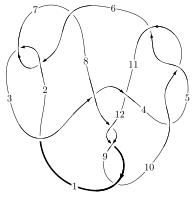
\includegraphics[width=112pt]{../../../GIT/diagram.site/Diagrams/png/1332_12a_0531.png}\\
\ \ \ A knot diagram\footnotemark}&
\allowdisplaybreaks
\textbf{Linearized knot diagam} \\
\cline{2-2}
 &
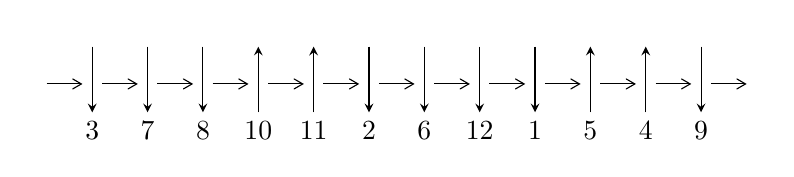
\begin{tikzpicture}[x=20pt, y=17pt]
	% nodes
	\node (C0) at (0, 0) {};
	\node (C1) at (1, 0) {};
	\node (C1U) at (1, +1) {};
	\node (C1D) at (1, -1) {3};

	\node (C2) at (2, 0) {};
	\node (C2U) at (2, +1) {};
	\node (C2D) at (2, -1) {7};

	\node (C3) at (3, 0) {};
	\node (C3U) at (3, +1) {};
	\node (C3D) at (3, -1) {8};

	\node (C4) at (4, 0) {};
	\node (C4U) at (4, +1) {};
	\node (C4D) at (4, -1) {10};

	\node (C5) at (5, 0) {};
	\node (C5U) at (5, +1) {};
	\node (C5D) at (5, -1) {11};

	\node (C6) at (6, 0) {};
	\node (C6U) at (6, +1) {};
	\node (C6D) at (6, -1) {2};

	\node (C7) at (7, 0) {};
	\node (C7U) at (7, +1) {};
	\node (C7D) at (7, -1) {6};

	\node (C8) at (8, 0) {};
	\node (C8U) at (8, +1) {};
	\node (C8D) at (8, -1) {12};

	\node (C9) at (9, 0) {};
	\node (C9U) at (9, +1) {};
	\node (C9D) at (9, -1) {1};

	\node (C10) at (10, 0) {};
	\node (C10U) at (10, +1) {};
	\node (C10D) at (10, -1) {5};

	\node (C11) at (11, 0) {};
	\node (C11U) at (11, +1) {};
	\node (C11D) at (11, -1) {4};

	\node (C12) at (12, 0) {};
	\node (C12U) at (12, +1) {};
	\node (C12D) at (12, -1) {9};
	\node (C13) at (13, 0) {};

	% arrows
	\draw[->,>={angle 60}]
	(C0) edge (C1) (C1) edge (C2) (C2) edge (C3) (C3) edge (C4) (C4) edge (C5) (C5) edge (C6) (C6) edge (C7) (C7) edge (C8) (C8) edge (C9) (C9) edge (C10) (C10) edge (C11) (C11) edge (C12) (C12) edge (C13) ;	\draw[->,>=stealth]
	(C1U) edge (C1D) (C2U) edge (C2D) (C3U) edge (C3D) (C4D) edge (C4U) (C5D) edge (C5U) (C6U) edge (C6D) (C7U) edge (C7D) (C8U) edge (C8D) (C9U) edge (C9D) (C10D) edge (C10U) (C11D) edge (C11U) (C12U) edge (C12D) ;
	\end{tikzpicture} \\
\hhline{~~} \\& 
\textbf{Solving Sequence} \\ \cline{2-2} 
 &
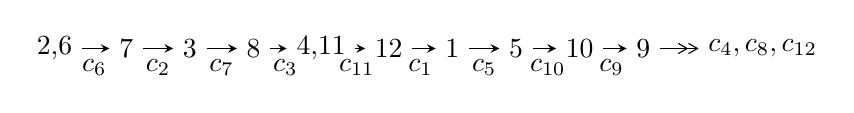
\begin{tikzpicture}[x=23pt, y=7pt]
	% node
	\node (A0) at (-1/8, 0) {2,6};
	\node (A1) at (1, 0) {7};
	\node (A2) at (2, 0) {3};
	\node (A3) at (3, 0) {8};
	\node (A4) at (65/16, 0) {4,11};
	\node (A5) at (41/8, 0) {12};
	\node (A6) at (49/8, 0) {1};
	\node (A7) at (57/8, 0) {5};
	\node (A8) at (65/8, 0) {10};
	\node (A9) at (73/8, 0) {9};
	\node (C1) at (1/2, -1) {$c_{6}$};
	\node (C2) at (3/2, -1) {$c_{2}$};
	\node (C3) at (5/2, -1) {$c_{7}$};
	\node (C4) at (7/2, -1) {$c_{3}$};
	\node (C5) at (37/8, -1) {$c_{11}$};
	\node (C6) at (45/8, -1) {$c_{1}$};
	\node (C7) at (53/8, -1) {$c_{5}$};
	\node (C8) at (61/8, -1) {$c_{10}$};
	\node (C9) at (69/8, -1) {$c_{9}$};
	\node (A10) at (11, 0) {$c_{4},c_{8},c_{12}$};

	% edge
	\draw[->,>=stealth]	
	(A0) edge (A1) (A1) edge (A2) (A2) edge (A3) (A3) edge (A4) (A4) edge (A5) (A5) edge (A6) (A6) edge (A7) (A7) edge (A8) (A8) edge (A9) ;
	\draw[->>,>={angle 60}]	
	(A9) edge (A10);
\end{tikzpicture} \\ 

\end{tabular} \\

\footnotetext{
The image of knot diagram is generated by the software ``\textbf{Draw programme}" developed by Andrew Bartholomew(\url{http://www.layer8.co.uk/maths/draw/index.htm\#Running-draw}), where we modified some parts for our purpose(\url{https://github.com/CATsTAILs/LinksPainter}).
}\phantom \\ \newline 
\centering \textbf{Ideals for irreducible components\footnotemark of $X_{\text{par}}$} 
 
\begin{align*}
I^u_{1}&=\langle 
1.50790\times10^{28} u^{83}-2.04992\times10^{28} u^{82}+\cdots+4.86000\times10^{27} b+2.90878\times10^{28},\\
\phantom{I^u_{1}}&\phantom{= \langle  }-5.01481\times10^{27} u^{83}+7.71256\times10^{27} u^{82}+\cdots+4.86000\times10^{27} a+1.48950\times10^{28},\;u^{84}-2 u^{83}+\cdots+8 u-1\rangle \\
I^u_{2}&=\langle 
u^2 a+2 a u-2 u^2+b+2 a-4 u-3,\;a^2-2 a u- u^2-2 a+6 u-1,\;u^3+u^2-1\rangle \\
I^u_{3}&=\langle 
b,\;a- u+1,\;u^3- u^2+1\rangle \\
\\
\end{align*}
\raggedright * 3 irreducible components of $\dim_{\mathbb{C}}=0$, with total 93 representations.\\
\footnotetext{All coefficients of polynomials are rational numbers. But the coefficients are sometimes approximated in decimal forms when there is not enough margin.}
\newpage
\renewcommand{\arraystretch}{1}
\centering \section*{I. $I^u_{1}= \langle 1.51\times10^{28} u^{83}-2.05\times10^{28} u^{82}+\cdots+4.86\times10^{27} b+2.91\times10^{28},\;-5.01\times10^{27} u^{83}+7.71\times10^{27} u^{82}+\cdots+4.86\times10^{27} a+1.49\times10^{28},\;u^{84}-2 u^{83}+\cdots+8 u-1 \rangle$}
\flushleft \textbf{(i) Arc colorings}\\
\begin{tabular}{m{7pt} m{180pt} m{7pt} m{180pt} }
\flushright $a_{2}=$&$\begin{pmatrix}0\\u\end{pmatrix}$ \\
\flushright $a_{6}=$&$\begin{pmatrix}1\\0\end{pmatrix}$ \\
\flushright $a_{7}=$&$\begin{pmatrix}1\\u^2\end{pmatrix}$ \\
\flushright $a_{3}=$&$\begin{pmatrix}- u\\- u^3+u\end{pmatrix}$ \\
\flushright $a_{8}=$&$\begin{pmatrix}- u^2+1\\u^2\end{pmatrix}$ \\
\flushright $a_{4}=$&$\begin{pmatrix}u^7-2 u^5+2 u^3-2 u\\- u^7+u^5-2 u^3+u\end{pmatrix}$ \\
\flushright $a_{11}=$&$\begin{pmatrix}1.03185 u^{83}-1.58695 u^{82}+\cdots-4.40283 u-3.06481\\-3.10267 u^{83}+4.21794 u^{82}+\cdots+29.3257 u-5.98515\end{pmatrix}$ \\
\flushright $a_{12}=$&$\begin{pmatrix}0.620344 u^{83}-0.533770 u^{82}+\cdots+1.10673 u-4.48153\\-2.17358 u^{83}+3.18151 u^{82}+\cdots+22.4583 u-4.80039\end{pmatrix}$ \\
\flushright $a_{1}=$&$\begin{pmatrix}u^3\\u^5- u^3+u\end{pmatrix}$ \\
\flushright $a_{5}=$&$\begin{pmatrix}2.85766 u^{83}-6.27375 u^{82}+\cdots-51.4385 u+14.7969\\2.17915 u^{83}-3.63605 u^{82}+\cdots-23.9333 u+5.83697\end{pmatrix}$ \\
\flushright $a_{10}=$&$\begin{pmatrix}6.60984 u^{83}-9.43458 u^{82}+\cdots-80.2900 u+17.7701\\1.88651 u^{83}-2.65258 u^{82}+\cdots-18.0252 u+4.01556\end{pmatrix}$ \\
\flushright $a_{9}=$&$\begin{pmatrix}5.50731 u^{83}-8.24850 u^{82}+\cdots-71.9841 u+16.5651\\0.919387 u^{83}-1.31392 u^{82}+\cdots-7.17730 u+2.14577\end{pmatrix}$\\&\end{tabular}
\flushleft \textbf{(ii) Obstruction class $= -1$}\\~\\
\flushleft \textbf{(iii) Cusp Shapes $= -0.957516 u^{83}+4.31532 u^{82}+\cdots+23.1863 u-1.43761$}\\~\\
\newpage\renewcommand{\arraystretch}{1}
\flushleft \textbf{(iv) u-Polynomials at the component}\newline \\
\begin{tabular}{m{50pt}|m{274pt}}
Crossings & \hspace{64pt}u-Polynomials at each crossing \\
\hline $$\begin{aligned}c_{1},c_{7}\end{aligned}$$&$\begin{aligned}
&u^{84}+28 u^{83}+\cdots+28 u+1
\end{aligned}$\\
\hline $$\begin{aligned}c_{2},c_{6}\end{aligned}$$&$\begin{aligned}
&u^{84}-2 u^{83}+\cdots+8 u-1
\end{aligned}$\\
\hline $$\begin{aligned}c_{3}\end{aligned}$$&$\begin{aligned}
&u^{84}+2 u^{83}+\cdots-4588 u-793
\end{aligned}$\\
\hline $$\begin{aligned}c_{4},c_{5},c_{10}\end{aligned}$$&$\begin{aligned}
&u^{84}+u^{83}+\cdots-40 u-8
\end{aligned}$\\
\hline $$\begin{aligned}c_{8},c_{9},c_{12}\end{aligned}$$&$\begin{aligned}
&u^{84}+4 u^{83}+\cdots+163 u-23
\end{aligned}$\\
\hline $$\begin{aligned}c_{11}\end{aligned}$$&$\begin{aligned}
&u^{84}-3 u^{83}+\cdots+1464 u-872
\end{aligned}$\\
\hline
\end{tabular}\\~\\
\newpage\renewcommand{\arraystretch}{1}
\flushleft \textbf{(v) Riley Polynomials at the component}\newline \\
\begin{tabular}{m{50pt}|m{274pt}}
Crossings & \hspace{64pt}Riley Polynomials at each crossing \\
\hline $$\begin{aligned}c_{1},c_{7}\end{aligned}$$&$\begin{aligned}
&y^{84}+60 y^{83}+\cdots-316 y+1
\end{aligned}$\\
\hline $$\begin{aligned}c_{2},c_{6}\end{aligned}$$&$\begin{aligned}
&y^{84}-28 y^{83}+\cdots-28 y+1
\end{aligned}$\\
\hline $$\begin{aligned}c_{3}\end{aligned}$$&$\begin{aligned}
&y^{84}-12 y^{83}+\cdots-50872888 y+628849
\end{aligned}$\\
\hline $$\begin{aligned}c_{4},c_{5},c_{10}\end{aligned}$$&$\begin{aligned}
&y^{84}-77 y^{83}+\cdots-64 y+64
\end{aligned}$\\
\hline $$\begin{aligned}c_{8},c_{9},c_{12}\end{aligned}$$&$\begin{aligned}
&y^{84}-78 y^{83}+\cdots-763 y+529
\end{aligned}$\\
\hline $$\begin{aligned}c_{11}\end{aligned}$$&$\begin{aligned}
&y^{84}+7 y^{83}+\cdots-34832832 y+760384
\end{aligned}$\\
\hline
\end{tabular}\\~\\
\newpage\flushleft \textbf{(vi) Complex Volumes and Cusp Shapes}
$$\begin{array}{c|c|c}  
\text{Solutions to }I^u_{1}& \I (\text{vol} + \sqrt{-1}CS) & \text{Cusp shape}\\
 \hline 
\begin{aligned}
u &= -1.005860 + 0.053427 I \\
a &= \phantom{-}1.18941 + 1.31282 I \\
b &= \phantom{-}1.213460 + 0.177851 I\end{aligned}
 & -0.638993 + 0.814219 I & \phantom{-0.000000 } 0 \\ \hline\begin{aligned}
u &= -1.005860 - 0.053427 I \\
a &= \phantom{-}1.18941 - 1.31282 I \\
b &= \phantom{-}1.213460 - 0.177851 I\end{aligned}
 & -0.638993 - 0.814219 I & \phantom{-0.000000 } 0 \\ \hline\begin{aligned}
u &= \phantom{-}1.009640 + 0.062094 I \\
a &= -0.30606 - 1.46538 I \\
b &= \phantom{-}0.119169 - 0.661433 I\end{aligned}
 & -3.80257 - 2.20400 I & \phantom{-0.000000 } 0 \\ \hline\begin{aligned}
u &= \phantom{-}1.009640 - 0.062094 I \\
a &= -0.30606 + 1.46538 I \\
b &= \phantom{-}0.119169 + 0.661433 I\end{aligned}
 & -3.80257 + 2.20400 I & \phantom{-0.000000 } 0 \\ \hline\begin{aligned}
u &= -0.776499 + 0.653312 I \\
a &= -0.222981 - 0.644766 I \\
b &= \phantom{-}0.153963 - 0.553953 I\end{aligned}
 & \phantom{-}0.07926 + 2.02066 I & \phantom{-0.000000 } 0 \\ \hline\begin{aligned}
u &= -0.776499 - 0.653312 I \\
a &= -0.222981 + 0.644766 I \\
b &= \phantom{-}0.153963 + 0.553953 I\end{aligned}
 & \phantom{-}0.07926 - 2.02066 I & \phantom{-0.000000 } 0 \\ \hline\begin{aligned}
u &= \phantom{-}0.695537 + 0.739243 I \\
a &= \phantom{-}1.61519 - 0.94961 I \\
b &= -1.345440 - 0.210053 I\end{aligned}
 & \phantom{-}4.80676 + 0.75078 I & \phantom{-0.000000 } 0 \\ \hline\begin{aligned}
u &= \phantom{-}0.695537 - 0.739243 I \\
a &= \phantom{-}1.61519 + 0.94961 I \\
b &= -1.345440 + 0.210053 I\end{aligned}
 & \phantom{-}4.80676 - 0.75078 I & \phantom{-0.000000 } 0 \\ \hline\begin{aligned}
u &= \phantom{-}0.624355 + 0.759958 I \\
a &= -1.325510 + 0.022658 I \\
b &= \phantom{-}0.772721 - 0.476917 I\end{aligned}
 & -2.12749 + 1.40116 I & \phantom{-0.000000 } 0 \\ \hline\begin{aligned}
u &= \phantom{-}0.624355 - 0.759958 I \\
a &= -1.325510 - 0.022658 I \\
b &= \phantom{-}0.772721 + 0.476917 I\end{aligned}
 & -2.12749 - 1.40116 I & \phantom{-0.000000 } 0\\
 \hline 
 \end{array}$$\newpage$$\begin{array}{c|c|c}  
\text{Solutions to }I^u_{1}& \I (\text{vol} + \sqrt{-1}CS) & \text{Cusp shape}\\
 \hline 
\begin{aligned}
u &= -0.728167 + 0.715851 I \\
a &= \phantom{-}3.24024 - 0.97356 I \\
b &= -1.51855 - 0.09042 I\end{aligned}
 & \phantom{-}5.33778 + 0.28990 I & \phantom{-0.000000 } 0 \\ \hline\begin{aligned}
u &= -0.728167 - 0.715851 I \\
a &= \phantom{-}3.24024 + 0.97356 I \\
b &= -1.51855 + 0.09042 I\end{aligned}
 & \phantom{-}5.33778 - 0.28990 I & \phantom{-0.000000 } 0 \\ \hline\begin{aligned}
u &= -0.688413 + 0.754788 I \\
a &= \phantom{-}0.551967 + 0.024503 I \\
b &= -0.262258 + 0.664682 I\end{aligned}
 & \phantom{-}1.80955 - 2.15614 I & \phantom{-0.000000 } 0 \\ \hline\begin{aligned}
u &= -0.688413 - 0.754788 I \\
a &= \phantom{-}0.551967 - 0.024503 I \\
b &= -0.262258 - 0.664682 I\end{aligned}
 & \phantom{-}1.80955 + 2.15614 I & \phantom{-0.000000 } 0 \\ \hline\begin{aligned}
u &= \phantom{-}0.976324\phantom{ +0.000000I} \\
a &= -0.614902\phantom{ +0.000000I} \\
b &= \phantom{-}1.53549\phantom{ +0.000000I}\end{aligned}
 & \phantom{-}0.457615\phantom{ +0.000000I} & -10.5000\phantom{ +0.000000I} \\ \hline\begin{aligned}
u &= \phantom{-}0.891298 + 0.536778 I \\
a &= \phantom{-}0.139782 + 0.390452 I \\
b &= -1.225720 - 0.173090 I\end{aligned}
 & \phantom{-}2.94410 - 0.08006 I & \phantom{-0.000000 } 0 \\ \hline\begin{aligned}
u &= \phantom{-}0.891298 - 0.536778 I \\
a &= \phantom{-}0.139782 - 0.390452 I \\
b &= -1.225720 + 0.173090 I\end{aligned}
 & \phantom{-}2.94410 + 0.08006 I & \phantom{-0.000000 } 0 \\ \hline\begin{aligned}
u &= -0.643339 + 0.823548 I \\
a &= -0.530313 + 0.337551 I \\
b &= \phantom{-}0.293170 - 0.790812 I\end{aligned}
 & -3.73484 - 5.86407 I & \phantom{-0.000000 } 0 \\ \hline\begin{aligned}
u &= -0.643339 - 0.823548 I \\
a &= -0.530313 - 0.337551 I \\
b &= \phantom{-}0.293170 + 0.790812 I\end{aligned}
 & -3.73484 + 5.86407 I & \phantom{-0.000000 } 0 \\ \hline\begin{aligned}
u &= -1.042210 + 0.126083 I \\
a &= -0.23452 - 1.89207 I \\
b &= -1.335370 - 0.268074 I\end{aligned}
 & \phantom{-}0.78059 + 5.59119 I & \phantom{-0.000000 } 0\\
 \hline 
 \end{array}$$\newpage$$\begin{array}{c|c|c}  
\text{Solutions to }I^u_{1}& \I (\text{vol} + \sqrt{-1}CS) & \text{Cusp shape}\\
 \hline 
\begin{aligned}
u &= -1.042210 - 0.126083 I \\
a &= -0.23452 + 1.89207 I \\
b &= -1.335370 + 0.268074 I\end{aligned}
 & \phantom{-}0.78059 - 5.59119 I & \phantom{-0.000000 } 0 \\ \hline\begin{aligned}
u &= \phantom{-}0.771829 + 0.720791 I \\
a &= \phantom{-}0.846377 + 0.082883 I \\
b &= -0.526872 + 0.345121 I\end{aligned}
 & \phantom{-}3.03488 - 1.28276 I & \phantom{-0.000000 } 0 \\ \hline\begin{aligned}
u &= \phantom{-}0.771829 - 0.720791 I \\
a &= \phantom{-}0.846377 - 0.082883 I \\
b &= -0.526872 - 0.345121 I\end{aligned}
 & \phantom{-}3.03488 + 1.28276 I & \phantom{-0.000000 } 0 \\ \hline\begin{aligned}
u &= \phantom{-}0.684662 + 0.805563 I \\
a &= -2.20441 + 0.70141 I \\
b &= \phantom{-}1.39828 + 0.26713 I\end{aligned}
 & \phantom{-}7.09037 + 5.56514 I & \phantom{-0.000000 } 0 \\ \hline\begin{aligned}
u &= \phantom{-}0.684662 - 0.805563 I \\
a &= -2.20441 - 0.70141 I \\
b &= \phantom{-}1.39828 - 0.26713 I\end{aligned}
 & \phantom{-}7.09037 - 5.56514 I & \phantom{-0.000000 } 0 \\ \hline\begin{aligned}
u &= \phantom{-}0.669349 + 0.848194 I \\
a &= \phantom{-}2.39133 - 0.39984 I \\
b &= -1.42903 - 0.31945 I\end{aligned}
 & \phantom{-}1.75823 + 9.89270 I & \phantom{-0.000000 } 0 \\ \hline\begin{aligned}
u &= \phantom{-}0.669349 - 0.848194 I \\
a &= \phantom{-}2.39133 + 0.39984 I \\
b &= -1.42903 + 0.31945 I\end{aligned}
 & \phantom{-}1.75823 - 9.89270 I & \phantom{-0.000000 } 0 \\ \hline\begin{aligned}
u &= -1.085550 + 0.056336 I \\
a &= -0.275785 + 0.475047 I \\
b &= -0.940188 + 0.467824 I\end{aligned}
 & -7.95233 + 0.71366 I & \phantom{-0.000000 } 0 \\ \hline\begin{aligned}
u &= -1.085550 - 0.056336 I \\
a &= -0.275785 - 0.475047 I \\
b &= -0.940188 - 0.467824 I\end{aligned}
 & -7.95233 - 0.71366 I & \phantom{-0.000000 } 0 \\ \hline\begin{aligned}
u &= \phantom{-}1.099610 + 0.112323 I \\
a &= \phantom{-}0.415514 + 1.063700 I \\
b &= -0.222123 + 0.831690 I\end{aligned}
 & -10.19880 - 5.33031 I & \phantom{-0.000000 } 0\\
 \hline 
 \end{array}$$\newpage$$\begin{array}{c|c|c}  
\text{Solutions to }I^u_{1}& \I (\text{vol} + \sqrt{-1}CS) & \text{Cusp shape}\\
 \hline 
\begin{aligned}
u &= \phantom{-}1.099610 - 0.112323 I \\
a &= \phantom{-}0.415514 - 1.063700 I \\
b &= -0.222123 - 0.831690 I\end{aligned}
 & -10.19880 + 5.33031 I & \phantom{-0.000000 } 0 \\ \hline\begin{aligned}
u &= -1.099630 + 0.155067 I \\
a &= -0.29211 + 1.63269 I \\
b &= \phantom{-}1.39491 + 0.34897 I\end{aligned}
 & -5.08068 + 9.58817 I & \phantom{-0.000000 } 0 \\ \hline\begin{aligned}
u &= -1.099630 - 0.155067 I \\
a &= -0.29211 - 1.63269 I \\
b &= \phantom{-}1.39491 - 0.34897 I\end{aligned}
 & -5.08068 - 9.58817 I & \phantom{-0.000000 } 0 \\ \hline\begin{aligned}
u &= \phantom{-}0.928621 + 0.619657 I \\
a &= -0.100165 - 1.173450 I \\
b &= \phantom{-}1.083530 - 0.032967 I\end{aligned}
 & \phantom{-}2.58787 - 4.44451 I & \phantom{-0.000000 } 0 \\ \hline\begin{aligned}
u &= \phantom{-}0.928621 - 0.619657 I \\
a &= -0.100165 + 1.173450 I \\
b &= \phantom{-}1.083530 + 0.032967 I\end{aligned}
 & \phantom{-}2.58787 + 4.44451 I & \phantom{-0.000000 } 0 \\ \hline\begin{aligned}
u &= \phantom{-}1.019450 + 0.457537 I \\
a &= -0.462210 - 0.527152 I \\
b &= \phantom{-}1.317910 + 0.341260 I\end{aligned}
 & -3.24713 + 2.82631 I & \phantom{-0.000000 } 0 \\ \hline\begin{aligned}
u &= \phantom{-}1.019450 - 0.457537 I \\
a &= -0.462210 + 0.527152 I \\
b &= \phantom{-}1.317910 - 0.341260 I\end{aligned}
 & -3.24713 - 2.82631 I & \phantom{-0.000000 } 0 \\ \hline\begin{aligned}
u &= -0.806273 + 0.783156 I \\
a &= -2.88994 + 0.82117 I \\
b &= \phantom{-}1.43003 + 0.12335 I\end{aligned}
 & \phantom{-}9.14541 + 2.98358 I & \phantom{-0.000000 } 0 \\ \hline\begin{aligned}
u &= -0.806273 - 0.783156 I \\
a &= -2.88994 - 0.82117 I \\
b &= \phantom{-}1.43003 - 0.12335 I\end{aligned}
 & \phantom{-}9.14541 - 2.98358 I & \phantom{-0.000000 } 0 \\ \hline\begin{aligned}
u &= -0.862705\phantom{ +0.000000I} \\
a &= \phantom{-}0.275443\phantom{ +0.000000I} \\
b &= \phantom{-}0.403590\phantom{ +0.000000I}\end{aligned}
 & -1.54513\phantom{ +0.000000I} & -4.21480\phantom{ +0.000000I}\\
 \hline 
 \end{array}$$\newpage$$\begin{array}{c|c|c}  
\text{Solutions to }I^u_{1}& \I (\text{vol} + \sqrt{-1}CS) & \text{Cusp shape}\\
 \hline 
\begin{aligned}
u &= -1.018780 + 0.525725 I \\
a &= -0.625001 + 0.295281 I \\
b &= -0.109685 + 0.817642 I\end{aligned}
 & -7.70761 + 1.33555 I & \phantom{-0.000000 } 0 \\ \hline\begin{aligned}
u &= -1.018780 - 0.525725 I \\
a &= -0.625001 - 0.295281 I \\
b &= -0.109685 - 0.817642 I\end{aligned}
 & -7.70761 - 1.33555 I & \phantom{-0.000000 } 0 \\ \hline\begin{aligned}
u &= -0.946108 + 0.648190 I \\
a &= \phantom{-}0.855038 - 0.839227 I \\
b &= -0.074916 - 0.634094 I\end{aligned}
 & -0.46603 + 3.04786 I & \phantom{-0.000000 } 0 \\ \hline\begin{aligned}
u &= -0.946108 - 0.648190 I \\
a &= \phantom{-}0.855038 + 0.839227 I \\
b &= -0.074916 + 0.634094 I\end{aligned}
 & -0.46603 - 3.04786 I & \phantom{-0.000000 } 0 \\ \hline\begin{aligned}
u &= \phantom{-}0.937402 + 0.690689 I \\
a &= -0.234099 - 0.621016 I \\
b &= \phantom{-}0.601970 + 0.256880 I\end{aligned}
 & \phantom{-}2.52543 - 4.12355 I & \phantom{-0.000000 } 0 \\ \hline\begin{aligned}
u &= \phantom{-}0.937402 - 0.690689 I \\
a &= -0.234099 + 0.621016 I \\
b &= \phantom{-}0.601970 - 0.256880 I\end{aligned}
 & \phantom{-}2.52543 + 4.12355 I & \phantom{-0.000000 } 0 \\ \hline\begin{aligned}
u &= \phantom{-}1.022020 + 0.590072 I \\
a &= \phantom{-}1.13586 + 1.40697 I \\
b &= -1.091450 + 0.410000 I\end{aligned}
 & -4.68766 - 5.74442 I & \phantom{-0.000000 } 0 \\ \hline\begin{aligned}
u &= \phantom{-}1.022020 - 0.590072 I \\
a &= \phantom{-}1.13586 - 1.40697 I \\
b &= -1.091450 - 0.410000 I\end{aligned}
 & -4.68766 + 5.74442 I & \phantom{-0.000000 } 0 \\ \hline\begin{aligned}
u &= -0.840965 + 0.836084 I \\
a &= \phantom{-}2.72881 - 0.61998 I \\
b &= -1.328120 - 0.208438 I\end{aligned}
 & \phantom{-}4.91735 + 5.68260 I & \phantom{-0.000000 } 0 \\ \hline\begin{aligned}
u &= -0.840965 - 0.836084 I \\
a &= \phantom{-}2.72881 + 0.61998 I \\
b &= -1.328120 + 0.208438 I\end{aligned}
 & \phantom{-}4.91735 - 5.68260 I & \phantom{-0.000000 } 0\\
 \hline 
 \end{array}$$\newpage$$\begin{array}{c|c|c}  
\text{Solutions to }I^u_{1}& \I (\text{vol} + \sqrt{-1}CS) & \text{Cusp shape}\\
 \hline 
\begin{aligned}
u &= -0.969325 + 0.683438 I \\
a &= -2.45171 + 1.35359 I \\
b &= \phantom{-}1.54495 - 0.07716 I\end{aligned}
 & \phantom{-}4.60204 + 5.08829 I & \phantom{-0.000000 } 0 \\ \hline\begin{aligned}
u &= -0.969325 - 0.683438 I \\
a &= -2.45171 - 1.35359 I \\
b &= \phantom{-}1.54495 + 0.07716 I\end{aligned}
 & \phantom{-}4.60204 - 5.08829 I & \phantom{-0.000000 } 0 \\ \hline\begin{aligned}
u &= \phantom{-}0.433786 + 0.682887 I \\
a &= -1.51254 - 0.21200 I \\
b &= \phantom{-}1.025860 + 0.318582 I\end{aligned}
 & -3.05008 + 0.92169 I & -4.35708 - 0.77356 I \\ \hline\begin{aligned}
u &= \phantom{-}0.433786 - 0.682887 I \\
a &= -1.51254 + 0.21200 I \\
b &= \phantom{-}1.025860 - 0.318582 I\end{aligned}
 & -3.05008 - 0.92169 I & -4.35708 + 0.77356 I \\ \hline\begin{aligned}
u &= \phantom{-}0.881987 + 0.801324 I \\
a &= -0.380306 + 0.465520 I \\
b &= \phantom{-}0.031624 - 0.527614 I\end{aligned}
 & \phantom{-}0.55770 - 2.99594 I & \phantom{-0.000000 } 0 \\ \hline\begin{aligned}
u &= \phantom{-}0.881987 - 0.801324 I \\
a &= -0.380306 - 0.465520 I \\
b &= \phantom{-}0.031624 + 0.527614 I\end{aligned}
 & \phantom{-}0.55770 + 2.99594 I & \phantom{-0.000000 } 0 \\ \hline\begin{aligned}
u &= -0.933284 + 0.748392 I \\
a &= \phantom{-}2.46322 - 1.14066 I \\
b &= -1.43177 + 0.10143 I\end{aligned}
 & \phantom{-}8.75543 + 2.78886 I & \phantom{-0.000000 } 0 \\ \hline\begin{aligned}
u &= -0.933284 - 0.748392 I \\
a &= \phantom{-}2.46322 + 1.14066 I \\
b &= -1.43177 - 0.10143 I\end{aligned}
 & \phantom{-}8.75543 - 2.78886 I & \phantom{-0.000000 } 0 \\ \hline\begin{aligned}
u &= \phantom{-}0.988622 + 0.690582 I \\
a &= -1.26017 - 2.60390 I \\
b &= \phantom{-}1.321940 - 0.243185 I\end{aligned}
 & \phantom{-}3.92465 - 6.21786 I & \phantom{-0.000000 } 0 \\ \hline\begin{aligned}
u &= \phantom{-}0.988622 - 0.690582 I \\
a &= -1.26017 + 2.60390 I \\
b &= \phantom{-}1.321940 + 0.243185 I\end{aligned}
 & \phantom{-}3.92465 + 6.21786 I & \phantom{-0.000000 } 0\\
 \hline 
 \end{array}$$\newpage$$\begin{array}{c|c|c}  
\text{Solutions to }I^u_{1}& \I (\text{vol} + \sqrt{-1}CS) & \text{Cusp shape}\\
 \hline 
\begin{aligned}
u &= -0.995284 + 0.694853 I \\
a &= -1.28752 + 0.63214 I \\
b &= \phantom{-}0.242296 + 0.706638 I\end{aligned}
 & \phantom{-}0.88560 + 7.67713 I & \phantom{-0.000000 } 0 \\ \hline\begin{aligned}
u &= -0.995284 - 0.694853 I \\
a &= -1.28752 - 0.63214 I \\
b &= \phantom{-}0.242296 - 0.706638 I\end{aligned}
 & \phantom{-}0.88560 - 7.67713 I & \phantom{-0.000000 } 0 \\ \hline\begin{aligned}
u &= \phantom{-}1.021630 + 0.682556 I \\
a &= \phantom{-}0.225119 + 0.797631 I \\
b &= -0.807645 - 0.537339 I\end{aligned}
 & -3.30063 - 6.88949 I & \phantom{-0.000000 } 0 \\ \hline\begin{aligned}
u &= \phantom{-}1.021630 - 0.682556 I \\
a &= \phantom{-}0.225119 - 0.797631 I \\
b &= -0.807645 + 0.537339 I\end{aligned}
 & -3.30063 + 6.88949 I & \phantom{-0.000000 } 0 \\ \hline\begin{aligned}
u &= -0.934862 + 0.804107 I \\
a &= -2.30600 + 1.00101 I \\
b &= \phantom{-}1.307880 - 0.193046 I\end{aligned}
 & \phantom{-}4.62756 + 0.42572 I & \phantom{-0.000000 } 0 \\ \hline\begin{aligned}
u &= -0.934862 - 0.804107 I \\
a &= -2.30600 - 1.00101 I \\
b &= \phantom{-}1.307880 + 0.193046 I\end{aligned}
 & \phantom{-}4.62756 - 0.42572 I & \phantom{-0.000000 } 0 \\ \hline\begin{aligned}
u &= \phantom{-}1.012340 + 0.716613 I \\
a &= \phantom{-}1.90120 + 2.49253 I \\
b &= -1.39597 + 0.28620 I\end{aligned}
 & \phantom{-}6.09591 - 11.29490 I & \phantom{-0.000000 } 0 \\ \hline\begin{aligned}
u &= \phantom{-}1.012340 - 0.716613 I \\
a &= \phantom{-}1.90120 - 2.49253 I \\
b &= -1.39597 - 0.28620 I\end{aligned}
 & \phantom{-}6.09591 + 11.29490 I & \phantom{-0.000000 } 0 \\ \hline\begin{aligned}
u &= -0.283981 + 0.692331 I \\
a &= -0.503996 - 0.319424 I \\
b &= \phantom{-}0.173149 + 0.760116 I\end{aligned}
 & -5.64015 + 3.06330 I & -7.15320 - 3.71038 I \\ \hline\begin{aligned}
u &= -0.283981 - 0.692331 I \\
a &= -0.503996 + 0.319424 I \\
b &= \phantom{-}0.173149 - 0.760116 I\end{aligned}
 & -5.64015 - 3.06330 I & -7.15320 + 3.71038 I\\
 \hline 
 \end{array}$$\newpage$$\begin{array}{c|c|c}  
\text{Solutions to }I^u_{1}& \I (\text{vol} + \sqrt{-1}CS) & \text{Cusp shape}\\
 \hline 
\begin{aligned}
u &= -1.035440 + 0.709315 I \\
a &= \phantom{-}1.36459 - 0.38464 I \\
b &= -0.304641 - 0.819504 I\end{aligned}
 & -4.92175 + 11.61130 I & \phantom{-0.000000 } 0 \\ \hline\begin{aligned}
u &= -1.035440 - 0.709315 I \\
a &= \phantom{-}1.36459 + 0.38464 I \\
b &= -0.304641 + 0.819504 I\end{aligned}
 & -4.92175 - 11.61130 I & \phantom{-0.000000 } 0 \\ \hline\begin{aligned}
u &= \phantom{-}0.196384 + 0.718380 I \\
a &= \phantom{-}2.39252 + 0.55518 I \\
b &= -1.366140 + 0.311678 I\end{aligned}
 & -0.77281 - 6.93544 I & -2.29673 + 5.13999 I \\ \hline\begin{aligned}
u &= \phantom{-}0.196384 - 0.718380 I \\
a &= \phantom{-}2.39252 - 0.55518 I \\
b &= -1.366140 - 0.311678 I\end{aligned}
 & -0.77281 + 6.93544 I & -2.29673 - 5.13999 I \\ \hline\begin{aligned}
u &= \phantom{-}1.035180 + 0.729097 I \\
a &= -2.15510 - 2.20542 I \\
b &= \phantom{-}1.43822 - 0.33088 I\end{aligned}
 & \phantom{-}0.6389 - 15.7800 I & \phantom{-0.000000 } 0 \\ \hline\begin{aligned}
u &= \phantom{-}1.035180 - 0.729097 I \\
a &= -2.15510 + 2.20542 I \\
b &= \phantom{-}1.43822 + 0.33088 I\end{aligned}
 & \phantom{-}0.6389 + 15.7800 I & \phantom{-0.000000 } 0 \\ \hline\begin{aligned}
u &= \phantom{-}0.185341 + 0.584468 I \\
a &= -2.26406 - 1.07778 I \\
b &= \phantom{-}1.352270 - 0.198800 I\end{aligned}
 & \phantom{-}4.67557 - 3.47099 I & \phantom{-}2.75649 + 4.83228 I \\ \hline\begin{aligned}
u &= \phantom{-}0.185341 - 0.584468 I \\
a &= -2.26406 + 1.07778 I \\
b &= \phantom{-}1.352270 + 0.198800 I\end{aligned}
 & \phantom{-}4.67557 + 3.47099 I & \phantom{-}2.75649 - 4.83228 I \\ \hline\begin{aligned}
u &= \phantom{-}0.492916 + 0.333326 I \\
a &= \phantom{-}0.555211 + 0.726800 I \\
b &= -1.300790 - 0.012081 I\end{aligned}
 & \phantom{-}3.26707 + 0.11469 I & \phantom{-}0.147841 + 0.385810 I \\ \hline\begin{aligned}
u &= \phantom{-}0.492916 - 0.333326 I \\
a &= \phantom{-}0.555211 - 0.726800 I \\
b &= -1.300790 + 0.012081 I\end{aligned}
 & \phantom{-}3.26707 - 0.11469 I & \phantom{-}0.147841 - 0.385810 I\\
 \hline 
 \end{array}$$\newpage$$\begin{array}{c|c|c}  
\text{Solutions to }I^u_{1}& \I (\text{vol} + \sqrt{-1}CS) & \text{Cusp shape}\\
 \hline 
\begin{aligned}
u &= \phantom{-}0.537371\phantom{ +0.000000I} \\
a &= -2.45205\phantom{ +0.000000I} \\
b &= \phantom{-}0.372992\phantom{ +0.000000I}\end{aligned}
 & -2.35654\phantom{ +0.000000I} & \phantom{-}3.13870\phantom{ +0.000000I} \\ \hline\begin{aligned}
u &= -0.208703 + 0.374292 I \\
a &= \phantom{-}0.716811 - 0.283596 I \\
b &= -0.169135 - 0.458913 I\end{aligned}
 & -0.132657 + 0.963114 I & -2.58462 - 6.99680 I \\ \hline\begin{aligned}
u &= -0.208703 - 0.374292 I \\
a &= \phantom{-}0.716811 + 0.283596 I \\
b &= -0.169135 + 0.458913 I\end{aligned}
 & -0.132657 - 0.963114 I & -2.58462 + 6.99680 I \\ \hline\begin{aligned}
u &= \phantom{-}0.230433\phantom{ +0.000000I} \\
a &= -3.01588\phantom{ +0.000000I} \\
b &= -1.37504\phantom{ +0.000000I}\end{aligned}
 & \phantom{-}3.21591\phantom{ +0.000000I} & \phantom{-}2.14730\phantom{ +0.000000I}\\
 \hline 
 \end{array}$$\newpage\newpage\renewcommand{\arraystretch}{1}
\centering \section*{II. $I^u_{2}= \langle u^2 a+2 a u-2 u^2+b+2 a-4 u-3,\;a^2-2 a u- u^2-2 a+6 u-1,\;u^3+u^2-1 \rangle$}
\flushleft \textbf{(i) Arc colorings}\\
\begin{tabular}{m{7pt} m{180pt} m{7pt} m{180pt} }
\flushright $a_{2}=$&$\begin{pmatrix}0\\u\end{pmatrix}$ \\
\flushright $a_{6}=$&$\begin{pmatrix}1\\0\end{pmatrix}$ \\
\flushright $a_{7}=$&$\begin{pmatrix}1\\u^2\end{pmatrix}$ \\
\flushright $a_{3}=$&$\begin{pmatrix}- u\\u^2+u-1\end{pmatrix}$ \\
\flushright $a_{8}=$&$\begin{pmatrix}- u^2+1\\u^2\end{pmatrix}$ \\
\flushright $a_{4}=$&$\begin{pmatrix}-1\\0\end{pmatrix}$ \\
\flushright $a_{11}=$&$\begin{pmatrix}a\\- u^2 a-2 a u+2 u^2-2 a+4 u+3\end{pmatrix}$ \\
\flushright $a_{12}=$&$\begin{pmatrix}- u^2 a-2 a u+2 u^2- a+4 u+3\\- u^2 a-2 a u+2 u^2-2 a+4 u+3\end{pmatrix}$ \\
\flushright $a_{1}=$&$\begin{pmatrix}- u^2+1\\u^2\end{pmatrix}$ \\
\flushright $a_{5}=$&$\begin{pmatrix}-2 u^2 a-4 a u+4 u^2-3 a+9 u+4\\2\end{pmatrix}$ \\
\flushright $a_{10}=$&$\begin{pmatrix}u^2 a+2 a u-2 u^2+a-4 u-3\\u^2 a+2 a u-2 u^2+2 a-4 u-3\end{pmatrix}$ \\
\flushright $a_{9}=$&$\begin{pmatrix}u^2 a+2 a u-3 u^2+a-4 u-2\\u^2 a+2 a u- u^2+2 a-4 u-3\end{pmatrix}$\\&\end{tabular}
\flushleft \textbf{(ii) Obstruction class $= 1$}\\~\\
\flushleft \textbf{(iii) Cusp Shapes $= -4 u-4$}\\~\\
\newpage\renewcommand{\arraystretch}{1}
\flushleft \textbf{(iv) u-Polynomials at the component}\newline \\
\begin{tabular}{m{50pt}|m{274pt}}
Crossings & \hspace{64pt}u-Polynomials at each crossing \\
\hline $$\begin{aligned}c_{1}\end{aligned}$$&$\begin{aligned}
&(u^3- u^2+2 u-1)^2
\end{aligned}$\\
\hline $$\begin{aligned}c_{2}\end{aligned}$$&$\begin{aligned}
&(u^3- u^2+1)^2
\end{aligned}$\\
\hline $$\begin{aligned}c_{3},c_{7}\end{aligned}$$&$\begin{aligned}
&(u^3+u^2+2 u+1)^2
\end{aligned}$\\
\hline $$\begin{aligned}c_{4},c_{5},c_{10}\\c_{11}\end{aligned}$$&$\begin{aligned}
&(u^2-2)^3
\end{aligned}$\\
\hline $$\begin{aligned}c_{6}\end{aligned}$$&$\begin{aligned}
&(u^3+u^2-1)^2
\end{aligned}$\\
\hline $$\begin{aligned}c_{8},c_{9}\end{aligned}$$&$\begin{aligned}
&(u+1)^6
\end{aligned}$\\
\hline $$\begin{aligned}c_{12}\end{aligned}$$&$\begin{aligned}
&(u-1)^6
\end{aligned}$\\
\hline
\end{tabular}\\~\\
\newpage\renewcommand{\arraystretch}{1}
\flushleft \textbf{(v) Riley Polynomials at the component}\newline \\
\begin{tabular}{m{50pt}|m{274pt}}
Crossings & \hspace{64pt}Riley Polynomials at each crossing \\
\hline $$\begin{aligned}c_{1},c_{3},c_{7}\end{aligned}$$&$\begin{aligned}
&(y^3+3 y^2+2 y-1)^2
\end{aligned}$\\
\hline $$\begin{aligned}c_{2},c_{6}\end{aligned}$$&$\begin{aligned}
&(y^3- y^2+2 y-1)^2
\end{aligned}$\\
\hline $$\begin{aligned}c_{4},c_{5},c_{10}\\c_{11}\end{aligned}$$&$\begin{aligned}
&(y-2)^6
\end{aligned}$\\
\hline $$\begin{aligned}c_{8},c_{9},c_{12}\end{aligned}$$&$\begin{aligned}
&(y-1)^6
\end{aligned}$\\
\hline
\end{tabular}\\~\\
\newpage\flushleft \textbf{(vi) Complex Volumes and Cusp Shapes}
$$\begin{array}{c|c|c}  
\text{Solutions to }I^u_{2}& \I (\text{vol} + \sqrt{-1}CS) & \text{Cusp shape}\\
 \hline 
\begin{aligned}
u &= -0.877439 + 0.744862 I \\
a &= \phantom{-}2.77766 - 0.30853 I \\
b &= -1.41421\phantom{ +0.000000I}\end{aligned}
 & \phantom{-}6.31400 + 2.82812 I & -0.49024 - 2.97945 I \\ \hline\begin{aligned}
u &= -0.877439 + 0.744862 I \\
a &= -2.53254 + 1.79826 I \\
b &= \phantom{-}1.41421\phantom{ +0.000000I}\end{aligned}
 & \phantom{-}6.31400 + 2.82812 I & -0.49024 - 2.97945 I \\ \hline\begin{aligned}
u &= -0.877439 - 0.744862 I \\
a &= \phantom{-}2.77766 + 0.30853 I \\
b &= -1.41421\phantom{ +0.000000I}\end{aligned}
 & \phantom{-}6.31400 - 2.82812 I & -0.49024 + 2.97945 I \\ \hline\begin{aligned}
u &= -0.877439 - 0.744862 I \\
a &= -2.53254 - 1.79826 I \\
b &= \phantom{-}1.41421\phantom{ +0.000000I}\end{aligned}
 & \phantom{-}6.31400 - 2.82812 I & -0.49024 + 2.97945 I \\ \hline\begin{aligned}
u &= \phantom{-}0.754878\phantom{ +0.000000I} \\
a &= \phantom{-}1.40822\phantom{ +0.000000I} \\
b &= \phantom{-}1.41421\phantom{ +0.000000I}\end{aligned}
 & \phantom{-}2.17641\phantom{ +0.000000I} & -7.01950\phantom{ +0.000000I} \\ \hline\begin{aligned}
u &= \phantom{-}0.754878\phantom{ +0.000000I} \\
a &= \phantom{-}2.10153\phantom{ +0.000000I} \\
b &= -1.41421\phantom{ +0.000000I}\end{aligned}
 & \phantom{-}2.17641\phantom{ +0.000000I} & -7.01950\phantom{ +0.000000I}\\
 \hline 
 \end{array}$$\newpage\newpage\renewcommand{\arraystretch}{1}
\centering \section*{III. $I^u_{3}= \langle b,\;a- u+1,\;u^3- u^2+1 \rangle$}
\flushleft \textbf{(i) Arc colorings}\\
\begin{tabular}{m{7pt} m{180pt} m{7pt} m{180pt} }
\flushright $a_{2}=$&$\begin{pmatrix}0\\u\end{pmatrix}$ \\
\flushright $a_{6}=$&$\begin{pmatrix}1\\0\end{pmatrix}$ \\
\flushright $a_{7}=$&$\begin{pmatrix}1\\u^2\end{pmatrix}$ \\
\flushright $a_{3}=$&$\begin{pmatrix}- u\\- u^2+u+1\end{pmatrix}$ \\
\flushright $a_{8}=$&$\begin{pmatrix}- u^2+1\\u^2\end{pmatrix}$ \\
\flushright $a_{4}=$&$\begin{pmatrix}1\\0\end{pmatrix}$ \\
\flushright $a_{11}=$&$\begin{pmatrix}u-1\\0\end{pmatrix}$ \\
\flushright $a_{12}=$&$\begin{pmatrix}u-1\\0\end{pmatrix}$ \\
\flushright $a_{1}=$&$\begin{pmatrix}u^2-1\\- u^2\end{pmatrix}$ \\
\flushright $a_{5}=$&$\begin{pmatrix}1\\0\end{pmatrix}$ \\
\flushright $a_{10}=$&$\begin{pmatrix}u-1\\0\end{pmatrix}$ \\
\flushright $a_{9}=$&$\begin{pmatrix}- u^2+u\\u^2\end{pmatrix}$\\&\end{tabular}
\flushleft \textbf{(ii) Obstruction class $= 1$}\\~\\
\flushleft \textbf{(iii) Cusp Shapes $= -4 u^2+10 u-8$}\\~\\
\newpage\renewcommand{\arraystretch}{1}
\flushleft \textbf{(iv) u-Polynomials at the component}\newline \\
\begin{tabular}{m{50pt}|m{274pt}}
Crossings & \hspace{64pt}u-Polynomials at each crossing \\
\hline $$\begin{aligned}c_{1},c_{3}\end{aligned}$$&$\begin{aligned}
&u^3- u^2+2 u-1
\end{aligned}$\\
\hline $$\begin{aligned}c_{2}\end{aligned}$$&$\begin{aligned}
&u^3+u^2-1
\end{aligned}$\\
\hline $$\begin{aligned}c_{4},c_{5},c_{10}\\c_{11}\end{aligned}$$&$\begin{aligned}
&u^3
\end{aligned}$\\
\hline $$\begin{aligned}c_{6}\end{aligned}$$&$\begin{aligned}
&u^3- u^2+1
\end{aligned}$\\
\hline $$\begin{aligned}c_{7}\end{aligned}$$&$\begin{aligned}
&u^3+u^2+2 u+1
\end{aligned}$\\
\hline $$\begin{aligned}c_{8},c_{9}\end{aligned}$$&$\begin{aligned}
&(u-1)^3
\end{aligned}$\\
\hline $$\begin{aligned}c_{12}\end{aligned}$$&$\begin{aligned}
&(u+1)^3
\end{aligned}$\\
\hline
\end{tabular}\\~\\
\newpage\renewcommand{\arraystretch}{1}
\flushleft \textbf{(v) Riley Polynomials at the component}\newline \\
\begin{tabular}{m{50pt}|m{274pt}}
Crossings & \hspace{64pt}Riley Polynomials at each crossing \\
\hline $$\begin{aligned}c_{1},c_{3},c_{7}\end{aligned}$$&$\begin{aligned}
&y^3+3 y^2+2 y-1
\end{aligned}$\\
\hline $$\begin{aligned}c_{2},c_{6}\end{aligned}$$&$\begin{aligned}
&y^3- y^2+2 y-1
\end{aligned}$\\
\hline $$\begin{aligned}c_{4},c_{5},c_{10}\\c_{11}\end{aligned}$$&$\begin{aligned}
&y^3
\end{aligned}$\\
\hline $$\begin{aligned}c_{8},c_{9},c_{12}\end{aligned}$$&$\begin{aligned}
&(y-1)^3
\end{aligned}$\\
\hline
\end{tabular}\\~\\
\newpage\flushleft \textbf{(vi) Complex Volumes and Cusp Shapes}
$$\begin{array}{c|c|c}  
\text{Solutions to }I^u_{3}& \I (\text{vol} + \sqrt{-1}CS) & \text{Cusp shape}\\
 \hline 
\begin{aligned}
u &= \phantom{-}0.877439 + 0.744862 I \\
a &= -0.122561 + 0.744862 I \\
b &= \phantom{-0.000000 } 0\end{aligned}
 & \phantom{-}1.37919 - 2.82812 I & -0.08593 + 2.22005 I \\ \hline\begin{aligned}
u &= \phantom{-}0.877439 - 0.744862 I \\
a &= -0.122561 - 0.744862 I \\
b &= \phantom{-0.000000 } 0\end{aligned}
 & \phantom{-}1.37919 + 2.82812 I & -0.08593 - 2.22005 I \\ \hline\begin{aligned}
u &= -0.754878\phantom{ +0.000000I} \\
a &= -1.75488\phantom{ +0.000000I} \\
b &= \phantom{-0.000000 } 0\end{aligned}
 & -2.75839\phantom{ +0.000000I} & -17.8280\phantom{ +0.000000I}\\
 \hline 
 \end{array}$$\newpage
\newpage\renewcommand{\arraystretch}{1}
\centering \section*{ IV. u-Polynomials}
\begin{tabular}{m{50pt}|m{274pt}}
Crossings & \hspace{64pt}u-Polynomials at each crossing \\
\hline $$\begin{aligned}c_{1}\end{aligned}$$&$\begin{aligned}
&((u^3- u^2+2 u-1)^3)(u^{84}+28 u^{83}+\cdots+28 u+1)
\end{aligned}$\\
\hline $$\begin{aligned}c_{2}\end{aligned}$$&$\begin{aligned}
&((u^3- u^2+1)^2)(u^3+u^2-1)(u^{84}-2 u^{83}+\cdots+8 u-1)
\end{aligned}$\\
\hline $$\begin{aligned}c_{3}\end{aligned}$$&$\begin{aligned}
&(u^3- u^2+2 u-1)(u^3+u^2+2 u+1)^2(u^{84}+2 u^{83}+\cdots-4588 u-793)
\end{aligned}$\\
\hline $$\begin{aligned}c_{4},c_{5},c_{10}\end{aligned}$$&$\begin{aligned}
&u^3(u^2-2)^3(u^{84}+u^{83}+\cdots-40 u-8)
\end{aligned}$\\
\hline $$\begin{aligned}c_{6}\end{aligned}$$&$\begin{aligned}
&(u^3- u^2+1)(u^3+u^2-1)^2(u^{84}-2 u^{83}+\cdots+8 u-1)
\end{aligned}$\\
\hline $$\begin{aligned}c_{7}\end{aligned}$$&$\begin{aligned}
&((u^3+u^2+2 u+1)^3)(u^{84}+28 u^{83}+\cdots+28 u+1)
\end{aligned}$\\
\hline $$\begin{aligned}c_{8},c_{9}\end{aligned}$$&$\begin{aligned}
&((u-1)^3)(u+1)^6(u^{84}+4 u^{83}+\cdots+163 u-23)
\end{aligned}$\\
\hline $$\begin{aligned}c_{11}\end{aligned}$$&$\begin{aligned}
&u^3(u^2-2)^3(u^{84}-3 u^{83}+\cdots+1464 u-872)
\end{aligned}$\\
\hline $$\begin{aligned}c_{12}\end{aligned}$$&$\begin{aligned}
&((u-1)^6)(u+1)^3(u^{84}+4 u^{83}+\cdots+163 u-23)
\end{aligned}$\\
\hline
\end{tabular}\newpage\renewcommand{\arraystretch}{1}
\centering \section*{ V. Riley Polynomials}
\begin{tabular}{m{50pt}|m{274pt}}
Crossings & \hspace{64pt}Riley Polynomials at each crossing \\
\hline $$\begin{aligned}c_{1},c_{7}\end{aligned}$$&$\begin{aligned}
&((y^3+3 y^2+2 y-1)^3)(y^{84}+60 y^{83}+\cdots-316 y+1)
\end{aligned}$\\
\hline $$\begin{aligned}c_{2},c_{6}\end{aligned}$$&$\begin{aligned}
&((y^3- y^2+2 y-1)^3)(y^{84}-28 y^{83}+\cdots-28 y+1)
\end{aligned}$\\
\hline $$\begin{aligned}c_{3}\end{aligned}$$&$\begin{aligned}
&((y^3+3 y^2+2 y-1)^3)(y^{84}-12 y^{83}+\cdots-5.08729\times10^{7} y+628849)
\end{aligned}$\\
\hline $$\begin{aligned}c_{4},c_{5},c_{10}\end{aligned}$$&$\begin{aligned}
&y^3(y-2)^6(y^{84}-77 y^{83}+\cdots-64 y+64)
\end{aligned}$\\
\hline $$\begin{aligned}c_{8},c_{9},c_{12}\end{aligned}$$&$\begin{aligned}
&((y-1)^9)(y^{84}-78 y^{83}+\cdots-763 y+529)
\end{aligned}$\\
\hline $$\begin{aligned}c_{11}\end{aligned}$$&$\begin{aligned}
&y^3(y-2)^6(y^{84}+7 y^{83}+\cdots-3.48328\times10^{7} y+760384)
\end{aligned}$\\
\hline
\end{tabular}
\vskip 2pc
\end{document}